\documentclass[12pt,a4paper]{article}
\usepackage[OT4]{polski}
\usepackage[utf8]{inputenc}
\usepackage{amssymb}
\usepackage[polish]{babel}
\usepackage{amsmath}
\usepackage{amsfonts}
\usepackage[left=3.5cm,right=2cm,top=2.5cm,bottom=2.5cm]{geometry}
\usepackage{graphicx}
\usepackage{indentfirst} 
\usepackage{float}
\usepackage{hyperref}

\hypersetup{
	colorlinks = true,
	linkcolor = black,
	filecolor = magenta,
	urlcolor = blue,
	}
\urlstyle{same}	
	
\author{Karpiński Maciej\\Radlak Piotr\\Wiecheć Sebastian\\\\\\\\\includegraphics[width=0.7\linewidth]{img/logoPWSZ.jpg}\\\\\\\\Projektowanie i programowanie systemów internetowych I}
\title{Projekt systemu zleceń mafijnych\\Mafia 2.0}

\begin{document}

	%Stron tytułowa
	\maketitle
	\thispagestyle{empty}
	\pagenumbering{arabic} 
	\clearpage

	%Spis treści
	\tableofcontents
	\newpage

	%Początek pierwszej sekcji opisującej system
	\section{Opis funkcjonalny systemu}
		Opis opis opis
	
	%Sekcja druga, opis wdrożonych kwalifikacji
	\section{Wdrożone kwalifikacje}
		
		Do zarządzania zależnościami wykorzystaliśmy menadżer pakietów NuGet.
		Wykorzystanie Bootstrapa zapewnia ostylowanie i RWD frontendu aplikacji ,,Mafia 2.0''.
		Zastosowanie EntityFramework w połączeniu z Microsoft SQL server zapewnia łączność z zewnętrzną bazą danych z systemem mapowania relacyjno-obiektowego (ORM).
		Dzięki zastosowaniu pakietu MailKit można z poziomu aplikacji łączyć się z serwerem pocztowym i wysyłać e-maile.
	
	%sekcja trzecia, opis wykorzystanych technologii
	\section{Opis technologiczny}
		Przy tworzeniu projektu ,,Mafia 2.0'' wykorzystano następujące technologie:

		\subsection{C\#}
			C\# jest obiektowym językiem programowania, zaprojektowanym w latach 1998 – 2001 dla firmy Microsoft.
			Napisany program jest kompilowany do Common Intermediate Language(CLI), który następnie wykonywany jest w środowisku uruchomieniowym takim jak .NET Framework,
			.NET Core, Mono lub DotGNU.
			Wykorzystanie CLI sprawia, że kod programu jest wieleplatformowy (dopóki istnieje odpowiednie środowisko uruchomieniowe).
			C\# posiada wiele wspólnych cech z językami Object Pascal, Delphi, C++ i Java a najważniejszymi cechami C\# są:
			\begin{itemize}
				\item Obiektowość z hierarchią o jednym elemencie nadrzędnym (podobnie jak w Javie);
				\item Zarządzaniem pamięcią zajmuje się środowisko uruchomieniowe;
				\item Właściwości i indeksery;
				\item Delegaty i zdarzenia – rozwinięcie wskaźników C++;
				\item Typy ogólne, generyczne, częściowe, Nullable, domniemane, anonimowe;
				\item Dynamiczne tworzenie kodu;
				\item Metody anonimowe;
				\item Wyrażenia lambda.
			\end{itemize}
			
		\subsection{ASP.NET Core}
			ASP.Net Core jest wysokowydajnym frameworkiem, do budowania nowoczesnych aplikacji internetowych wykorzystujących moc obliczeniową chmur. ASP.Net Core jest technologią open - source,
			wykorzystującą silnik html Razor, dzięki której możliwe jest tworzenie aplikacji mulitplaformowych, które mogą być używane na każdym urządzeniu wyposażonym w przeglądarkę
			internetową.
			
		\subsection{Bootstrap}		
			Bootstrap jest frameworkiem CSS, który koncentruje się na uproszczeniu tworzenia frontendu stron internetowych. Rezultatem dodania Bootstrapa do projektu jest jednolity wygląd
			wszystkich elementów interfejsów we wszystkich przeglądarkach. Dodatkowo programiści mogą skorzystać z klas w CSS w celu dalszego dostosowywania wyglądu ich zawartości. Bootstrap
			zawiera kilka składników JavaScript, które zapewniają dodatkowe elementy interfejsu użytkownika, takie jak okna dialogowe, podpowiedzi czy karuzele. 

		\subsection{Entity Framework}		 
		 Entity Framework jest technologią open source do mapowania obiektowo – relacyjnego (ORM), które wspierają rozwój aplikacji zorientowanych na dane.
		 Entity Framework umożliwia programistom pracę z danymi w postaci obiektów i właściwości specyficznych dla domeny, bez konieczności przejmowania się bazowymi
		 tabelami i kolumnami baz danych, w których dane są przechowywane. 

		\subsection{MSSQL}		 
		 	Microsoft SQL Server jest systemem zarządzania relacyjnymi bazami danych opracowany przez firmę Microsoft. Cechą charakterystyczną jest wykorzystanie głównie język zapytań
		 	Transact-SQL, który jest rozwinięciem standardu ANSI/ISO. W projekcie wykorzystano wersje 2019 Express, która jest bezpłatną edycją programu Microsoft SQL Server, oferująca
		 	podstawowy silnik bazy danych, nieposiadający ograniczenia ilości obsługiwanych baz danych lub użytkowników. Ograniczenia, występujące w wersji Express to  m. in.:
		 	korzystanie z jednego procesora, 1 GB pamięci RAM, 10GB plików bazy danych czy brak SQL Agent.
		
		\subsection{MailKit}
			MailKit jest multiplatformową otwarto źródłową biblioteką .NET klienta pocztowego opartą o MimeKit, która została zoptymalizowana pod kątem urządzeń mobilnych.\\
			MailKit oferuje funkcjonalność:
			\begin{itemize}
				\item Obsługa proxy HTTP, Socks4, Socks4a i Socks5.
				\item Uwierzytelnianie SASL.
				\item Kompletny klient SMTP.
				\item Kompletny klient POP3.
				\item Kompletny klient IMAP.
				\item Sortowanie i wątkowanie wiadomości po stronie klienta.
				\item Asynchroniczne wersje wszystkich metod sieciowych.
				\item Obsługa S/MIME, OpenPGP, DKIM i ARC.
				\item Obsługa Microsoft TNEF.
			\end{itemize}
		\subsection{Node.js}
			Node.js jest otwarto źródłowym, wieloplatformowym środowiskiem uruchomieniowym JavaScript, które wykonuje kod poza przeglądarką internetową. Node.js pozwala programistom pisać 					narzędzia wiersza poleceń oraz skrypty po stronie serwera, które wygenerują zawartość strony internetowej przed jej wysłaniem do przeglądarki internetowej użytkownika. Node.js 					reprezentuje paradygmat ,,JavaScript wszędzie'', który ujednolica tworzenie aplikacji internetowych wokół jednego języka programowania. 
		
	%Sekcja czwarta, instrukcja lokalnego i zdalnego uruchomienia systemu
	\section{Instrukcja lokalnego i zdalnego uruchomienia systemu}
		\subsection{Lokalne uruchomienie systemu}
			Do uruchomienia Systemu zleceń mafijnych Mafia 2.0 wymagane jest następujące oprogramowanie:
			\begin{itemize}
				\item Microsoft Windows 10
				\item ASP.NET Core Runtime 3.1.3 Hosting Bundle (Dołączony do instalatora)
				\item Microsoft SQL Server 2019 Express Edition (Dołączony do instalatora)
				\item SQL Server Management Studio (SSMS)
			\end{itemize}
			Uwaga: Cały proces instalacji należy wykonać z uprawnieniami administratora!\\
			Instalacja:
			\begin{enumerate}
				\item \href{https://github.com/p10trek/PAM2Zaliczenie/releases}{Ze strony projektu} (\url{https://github.com/p10trek/PAM2Zaliczenie/releases}) należy pobrać plik
						,,PAM\_Killers\_Local\_Setup.exe'';
				\item Postępować zgodnie z wytycznymi kreatora instalacji;
				\begin{figure}[H]
					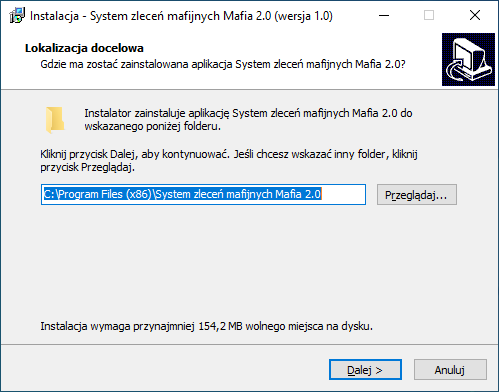
\includegraphics[scale=0.5]{img/Local_Install_1.png}
					\centering
				\end{figure}
				\item Po ukończeniu instalacji aplikacji, kreator zaproponuje instalację wymaganych do działania składników;
					\begin{figure}[H]
						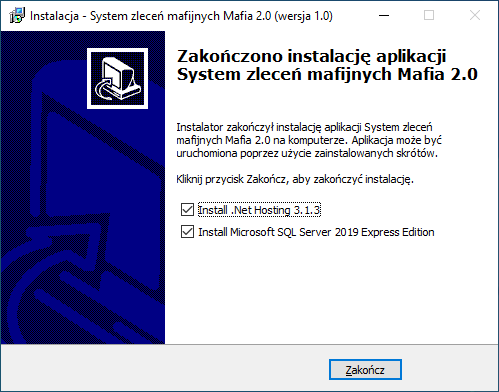
\includegraphics[scale=0.5]{img/Local_Install_2.png}
						\centering
					\end{figure}		
				\item Zainstalować ASP.NET Core Runtime 3.1.3 Hosting Bundle (można pominąć jeśli jest już zainstalowane);
					\begin{figure}[H]
						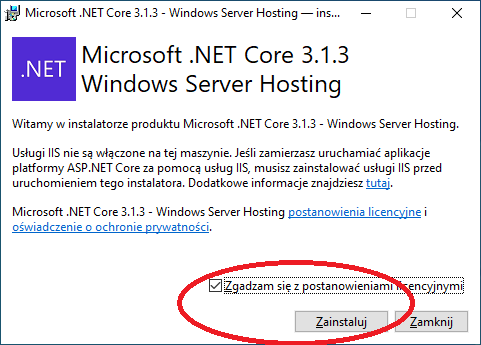
\includegraphics[scale=0.5]{img/Local_Install_3.png}
						\centering
					\end{figure}
				\item Zainstalować Microsoft SQL Server 2019 Express Edition, wybierając wersję instalacji: ,,Basic'' (można pominąć jeśli jest już zainstalowane);
					\begin{figure}[H]
						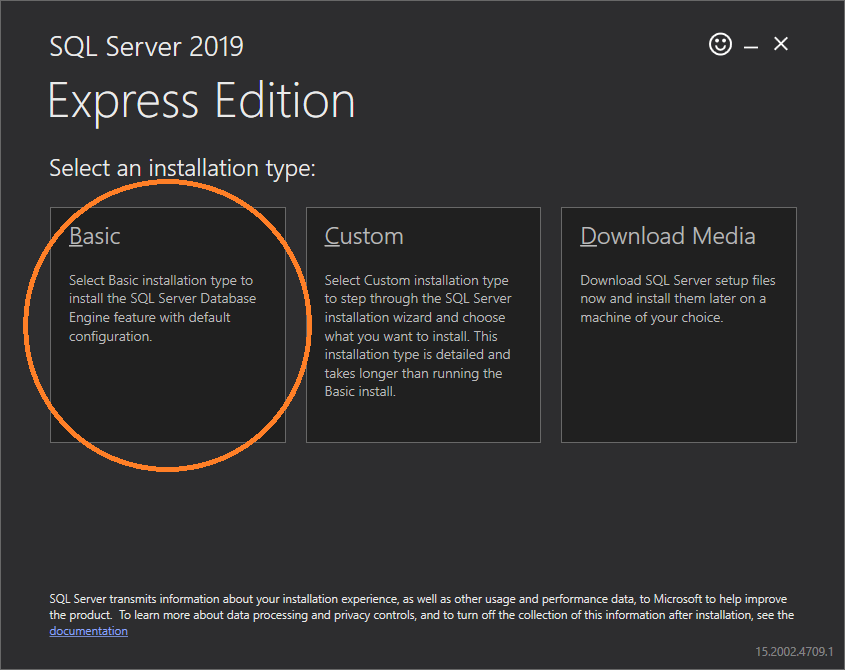
\includegraphics[scale=0.3]{img/Local_Install_4.png}
						\centering
					\end{figure}
				\item Po zakończeniu instalacji serwera SQL, można przejść do strony pobierania aplikacji SQL Server Management Studio (1. Install SSMS) albo zakończyć działanie instalatora (2. 						Close)
					\begin{figure}[H]
						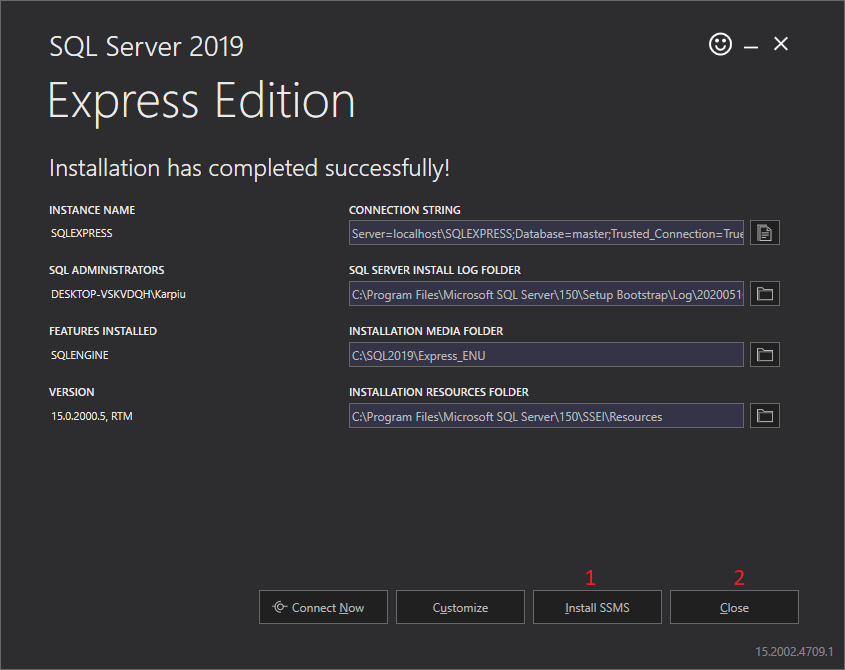
\includegraphics[scale=0.3]{img/Local_Install_5.png}
						\centering
					\end{figure}				
				\item \href{https://docs.microsoft.com/en-us/sql/ssms/download-sql-server-management-studio-ssms}{Pobrać ze strony internetowej instalator SQL Server Management Studio (SSMS)}
						\url{https://tiny.pl/77hn7} 
					\begin{figure}[H]
						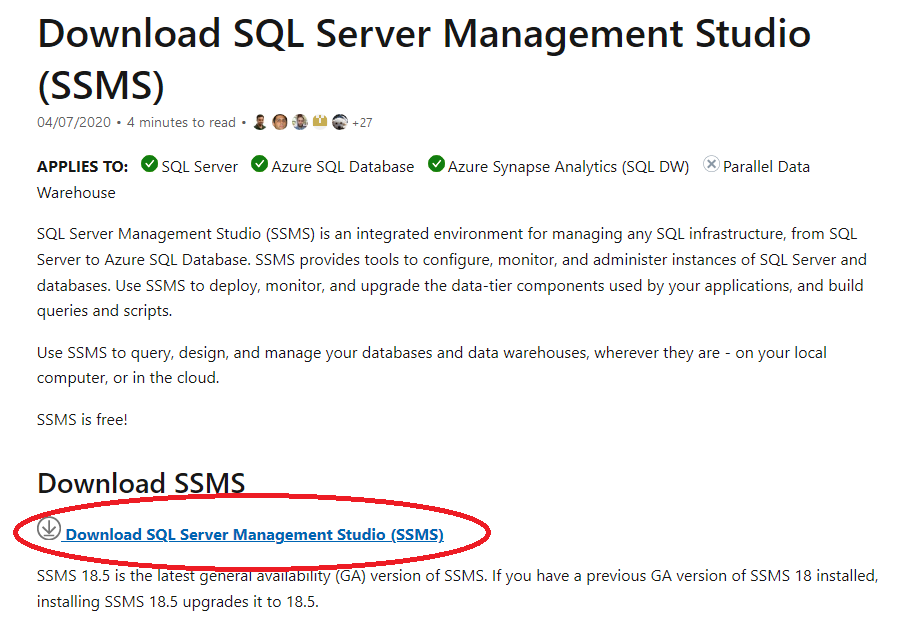
\includegraphics[scale=0.3]{img/Local_Install_5.5.png}
						\centering
					\end{figure}				
				\item Uruchomić pobrany plik i zainstalować SQL Server Management Studio;
					\begin{figure}[H]
						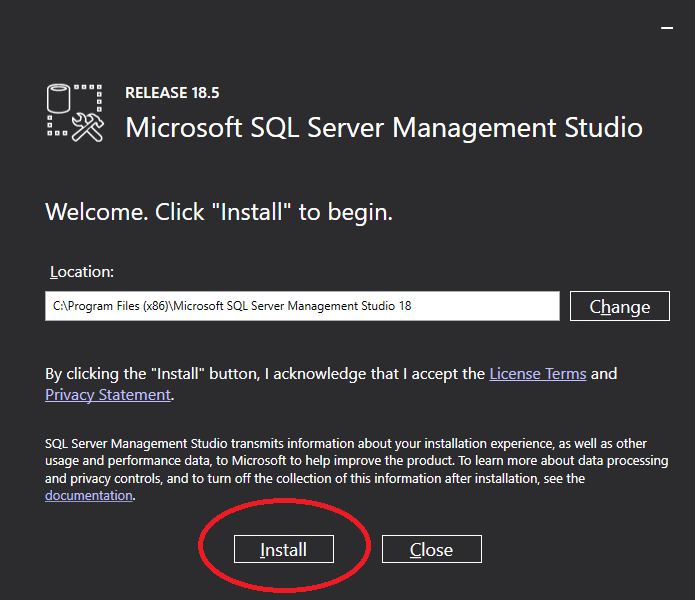
\includegraphics[scale=0.34]{img/Local_Install_6.png}
						\centering
					\end{figure}
				\item Po ukończeniu instalacji SQL Server Management Studio należy uruchomić ponownie system;
					\begin{figure}[H]
						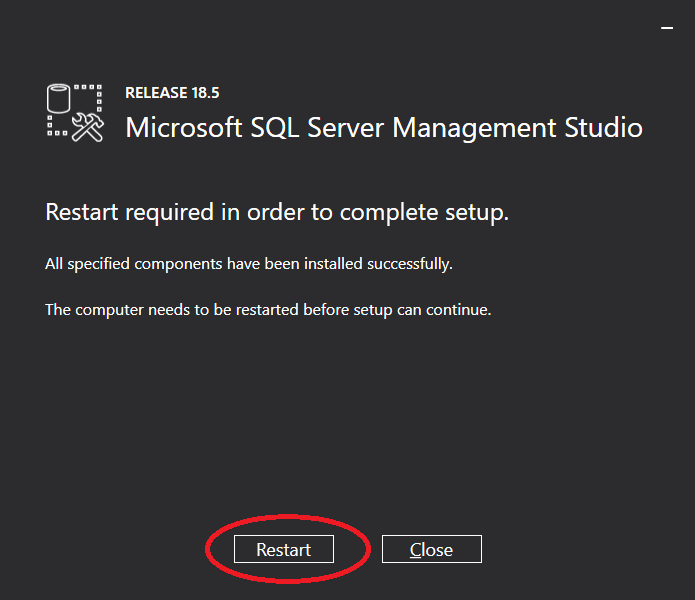
\includegraphics[scale=0.4]{img/Local_Install_7.png}
						\centering
					\end{figure}
				\item Z menu ,,Start'' Uruchomić Microsoft SQL Server Management Studio 18;
					\begin{figure}[H]
						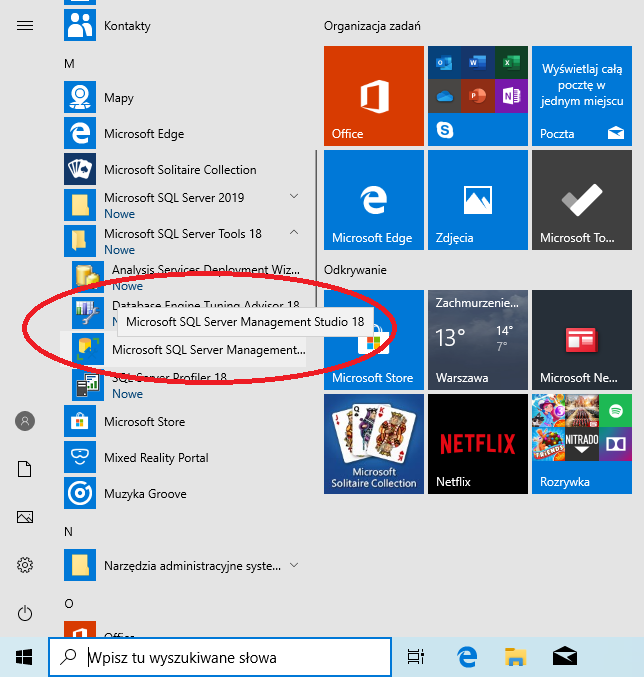
\includegraphics[scale=0.4]{img/Local_Install_8.png}
						\centering
					\end{figure}		
				\item Połączyć się z lokalną bazą danych (Pola ,,Server name'' oraz ,,User name'' mogą się różnić);
					\begin{figure}[H]
						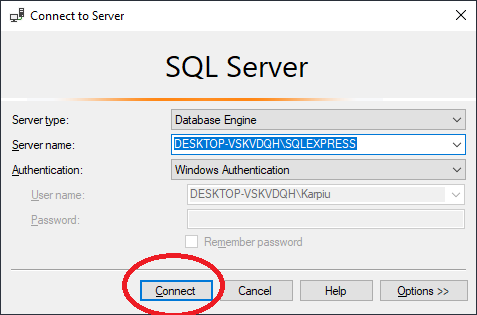
\includegraphics[scale=0.4]{img/Local_Install_9.png}
						\centering
					\end{figure}	
				\item Po podłączeniu do bazy danych należy rozwinąć listę składników bazy danych a następnie przy pomocy prawego przycisku myszy należy wybrać pole ,,Databases'' i wybrać 									Restore Database...''\\
					\begin{figure}[H]
						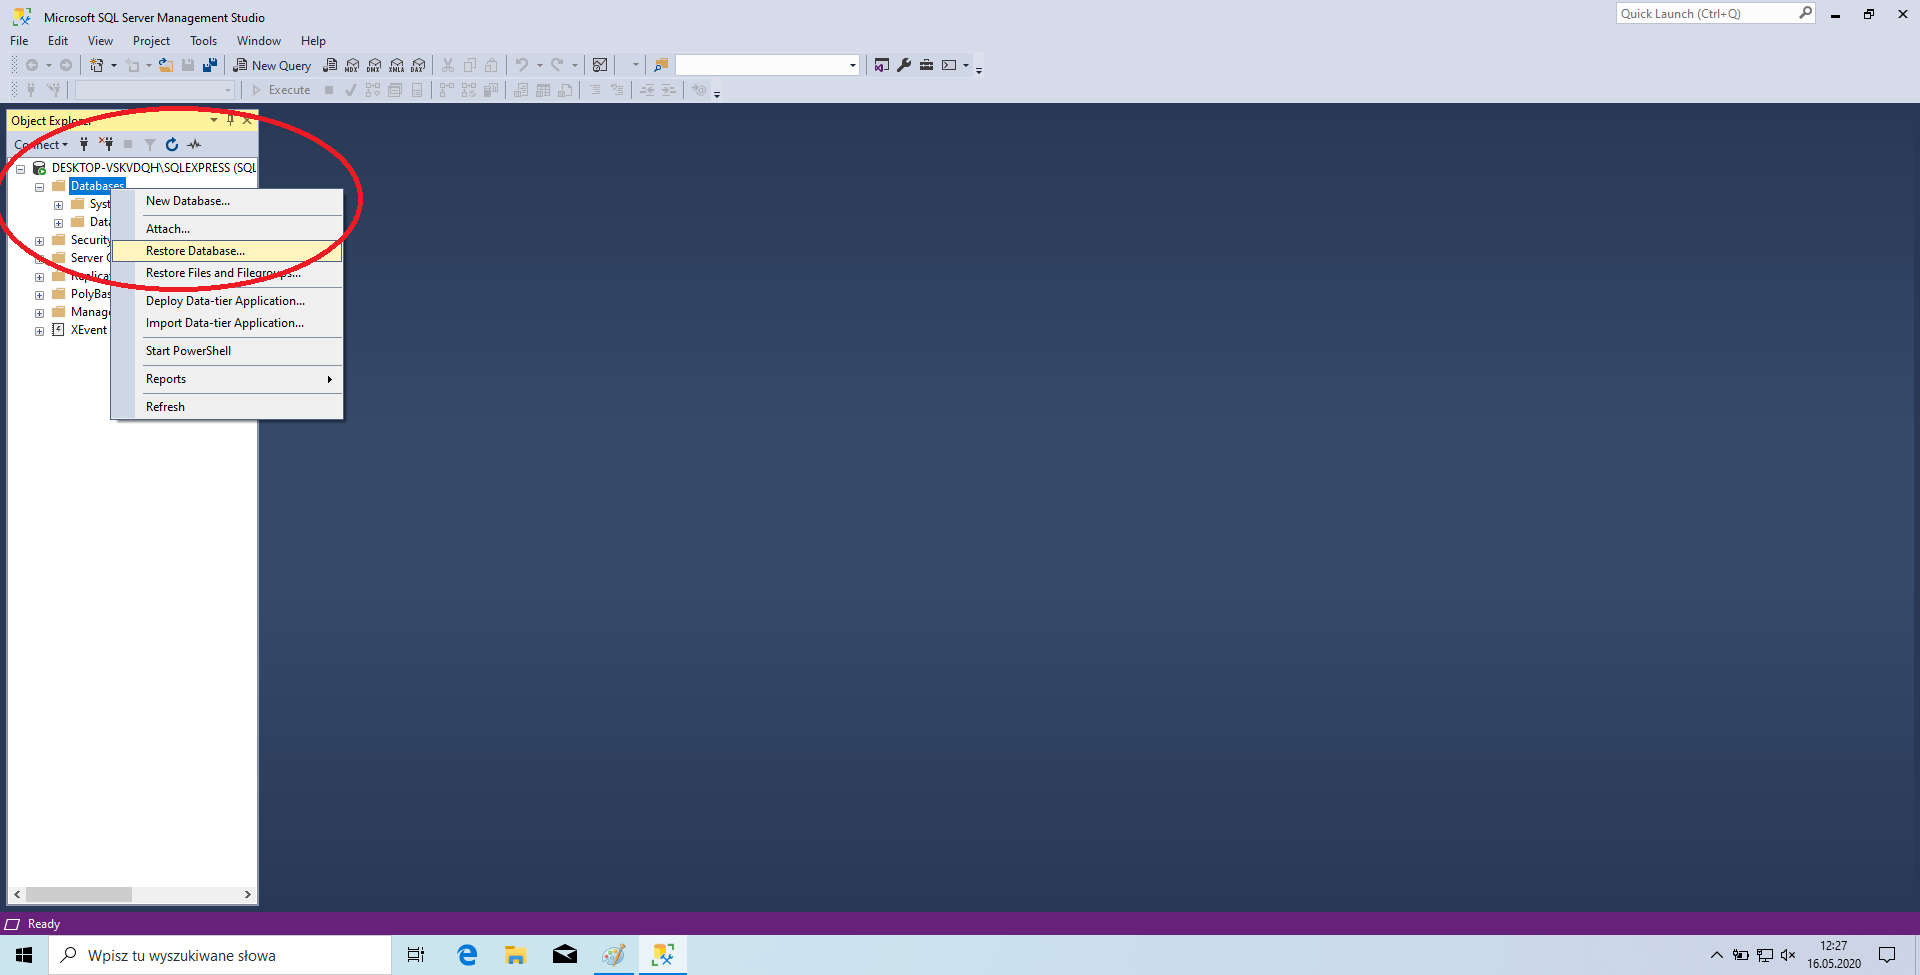
\includegraphics[scale=0.3]{img/Local_Install_10.png}
						\centering
					\end{figure}				 					
				\item Przywrócić bazę danych z pliku o nazwie ,,PAM\_KillersDB.bak'' znajdującego się na lokalnym dysku ,,C:$\backslash$'';
					\begin{figure}[H]
					
						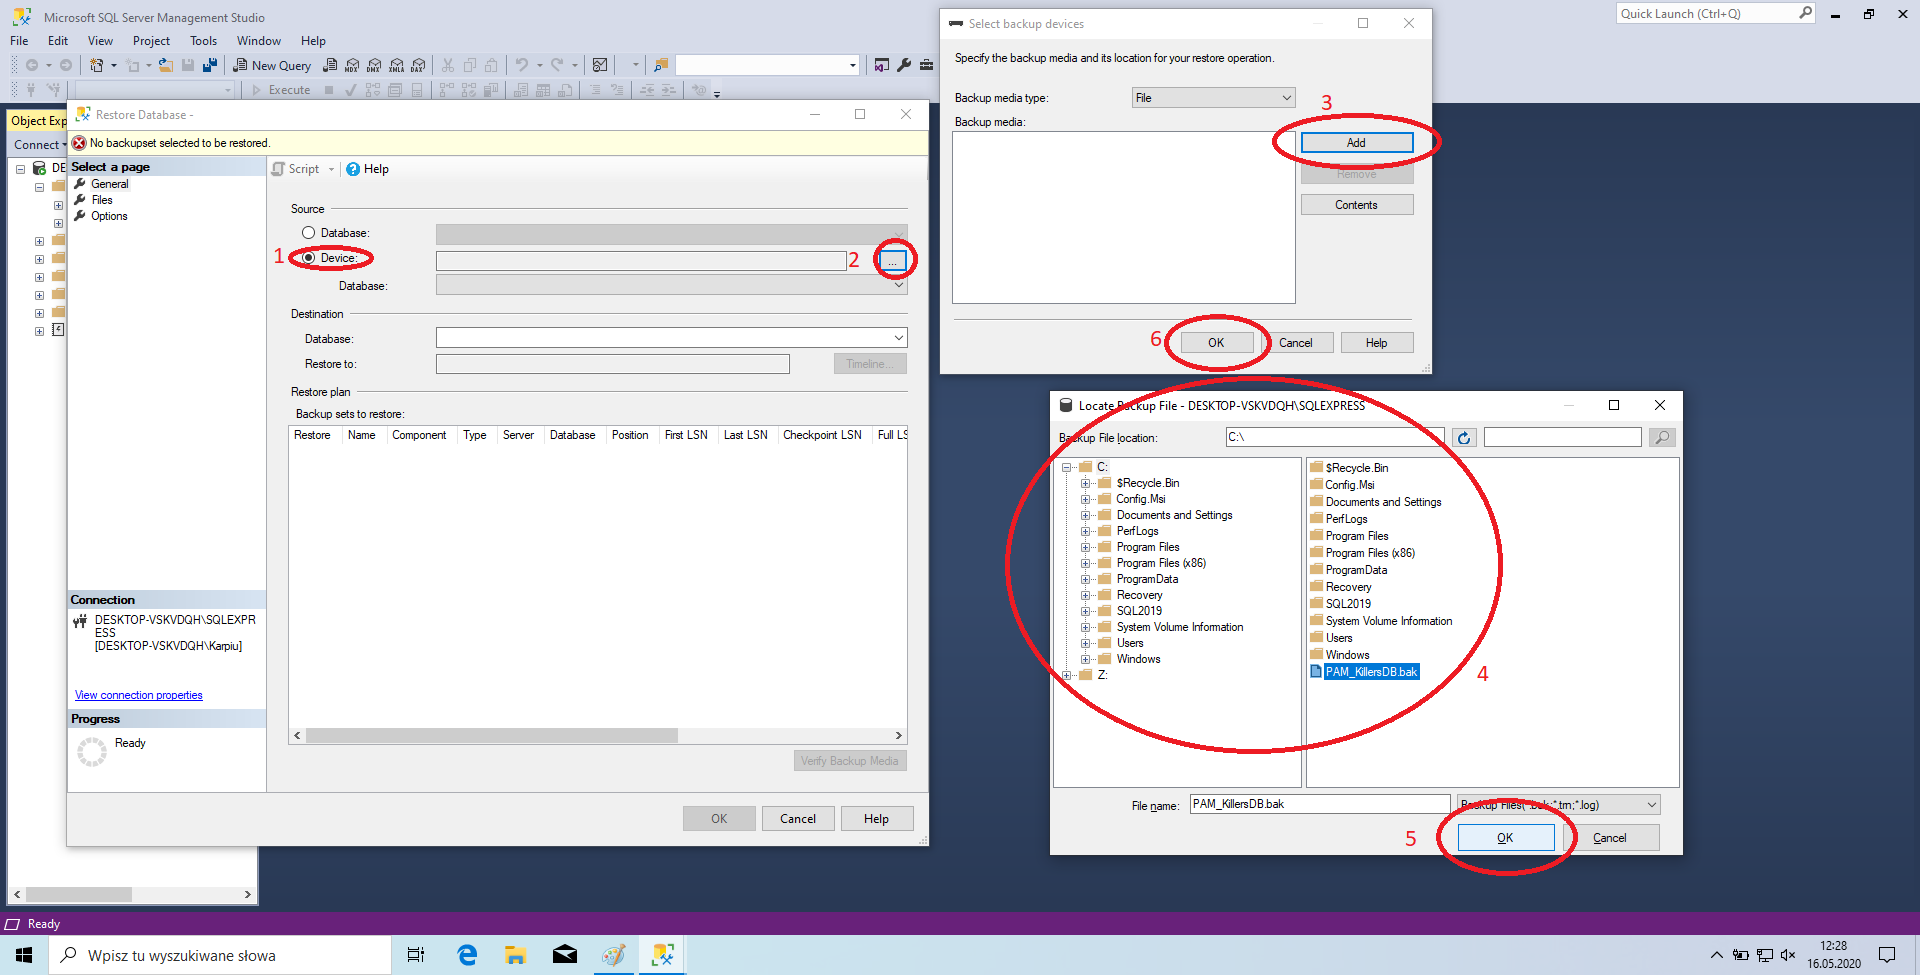
\includegraphics[scale=0.3]{img/Local_Install_11.png}\\
						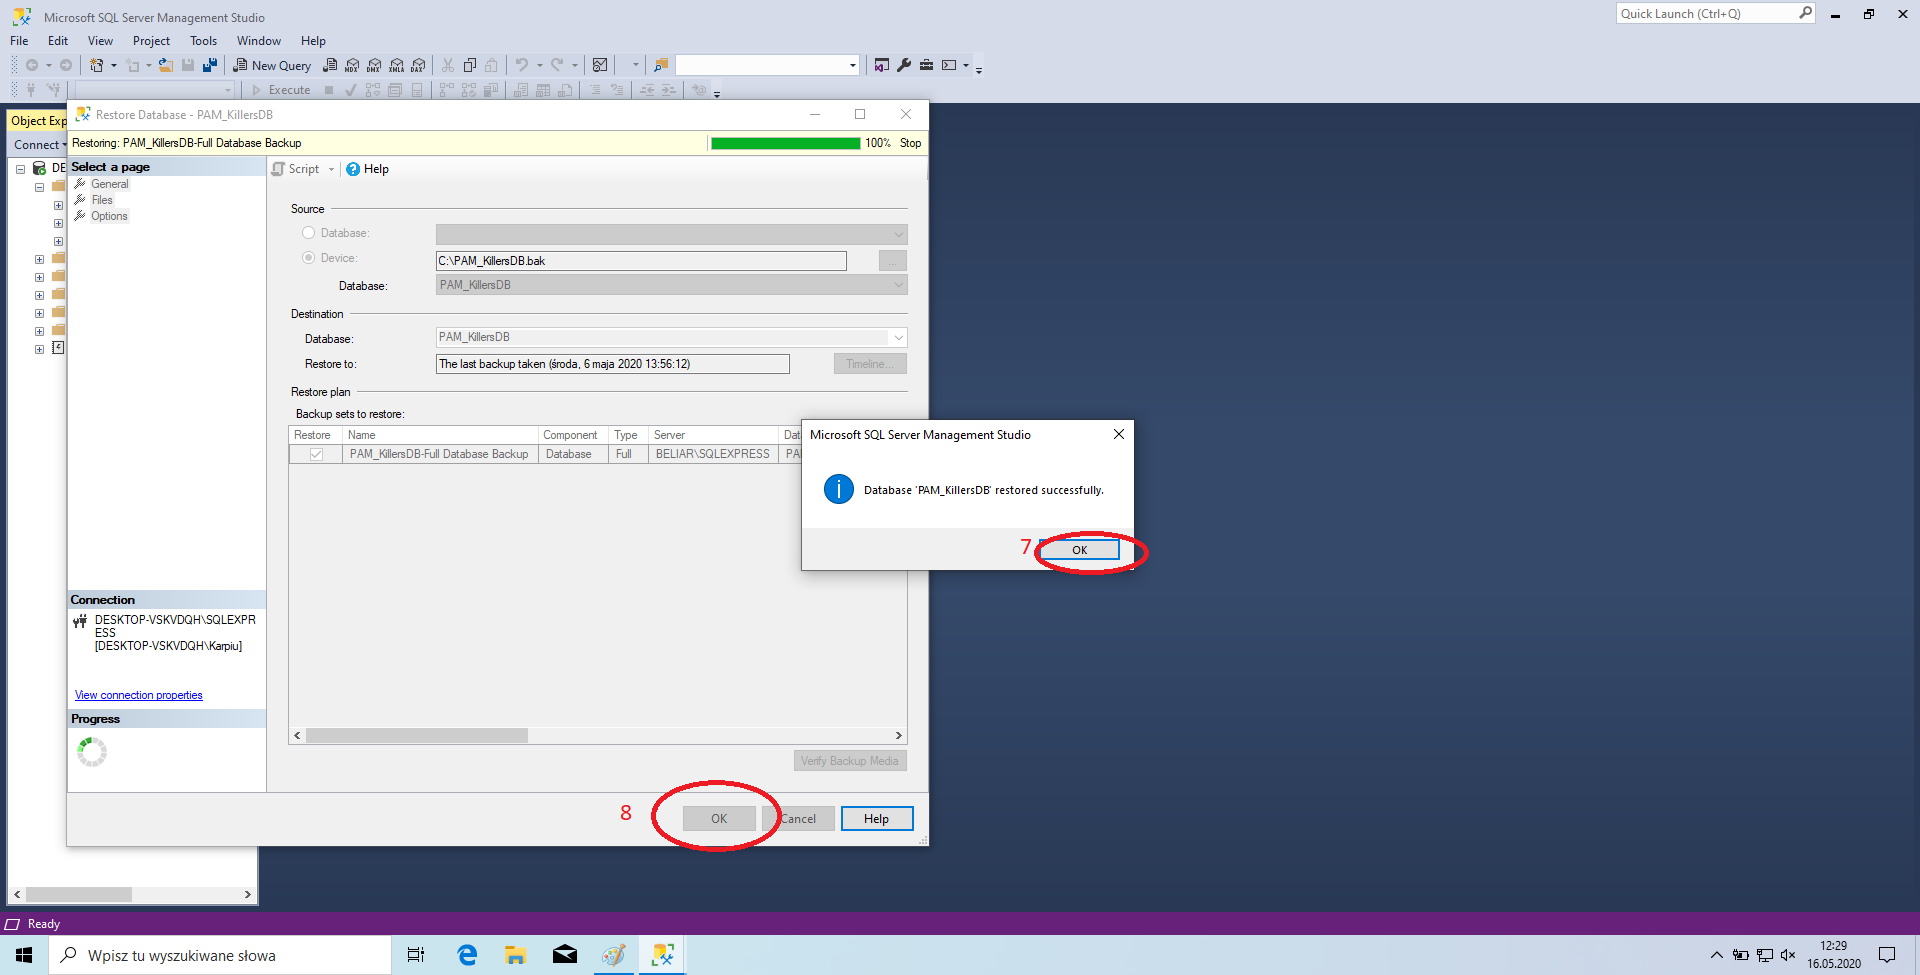
\includegraphics[scale=0.3]{img/Local_Install_12.png}
						\centering
						
					\end{figure}				
				\item Przy pomocy aplikacji ,,Notatnik'' należy edytować plik ,,appsettings.json'' znajdujący się w głównym katalogu aplikacji (Domyślnie:
						,,C:$\backslash$Program Files$\backslash$System zleceń mafijnych Mafia 2.0'') i zmienić wartości w sekcji ,,EmailConfiguration'', zgodnie z ustawieniami podanymi 									przez administratora serwera pocztowego;\\
					\begin{figure}[H]
						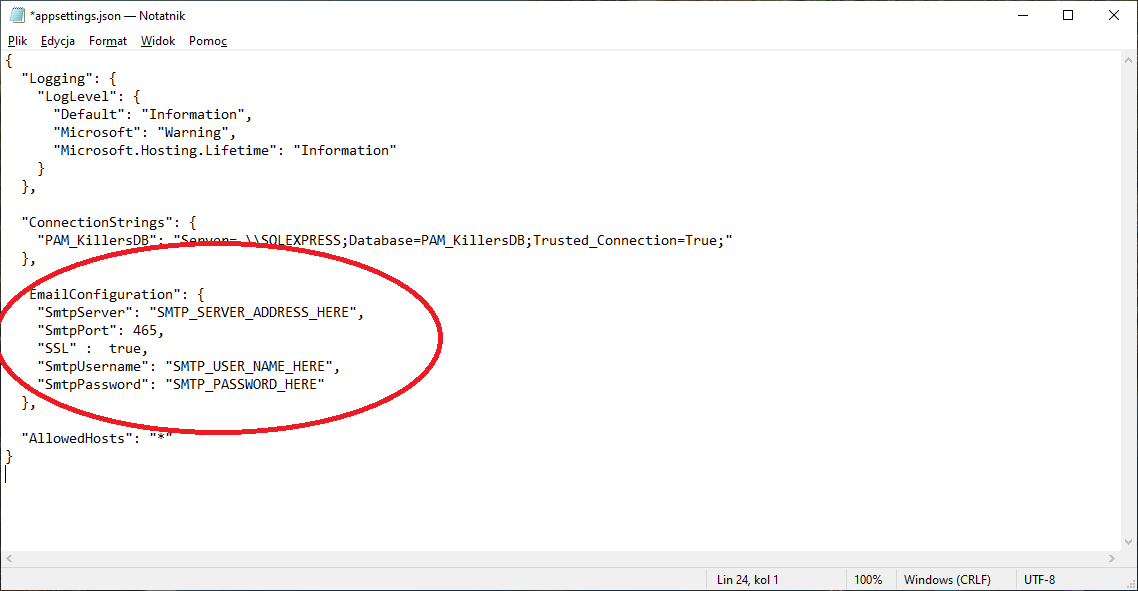
\includegraphics[scale=0.5]{img/Local_Install_13.png}
						\centering
					\end{figure}				
				\item Uruchomić ponownie system.
			\end{enumerate}
			System zleceń mafijnych ,,Mafia 2.0'' jest gotowy do używania na lokalnym komputerze. Aby uruchomić aplikację należy użyć skrótu w menu ,,Start'' lub na Pulpicie (jeżeli została 						zaznaczona odpowiednia opcja w czasie instalacji). W zależności od mocy obliczeniowej używanego komputera pierwsze uruchomienie aplikacji po starcie systemu operacyjnego
				może trwać dłużej.		
		\subsection{Zdalne uruchomienie systemu}
			Do uruchomienia Systemu zleceń mafijnych Mafia 2.0 wymagane jest następujące oprogramowanie:
			\begin{itemize}
				\item Linux Ubuntu 18.04 LTS 64bit.
				\item 2GB RAM
			\end{itemize}
			
			\begin{enumerate}
					
			\item Za pomocą polecenia:\\
			
			\fbox{wget -O - https://github.com/Karpfly2822/Test-VS-Repo/releases/download/1/PAM\_Linux\_Installer.sh | bash }
			nastąpi pobranie i instalacja wszystkich wymaganaych pakietów i aplikacji systemu zleceń.\\
			\item Po zakończeniu skryptu należy przeprowadzić konfigurację bazy danych MSSQL:	\\
			\fbox{sudo /opt/mssql/bin/mssql-conf setup\\
			/opt/mssql-tools/bin/sqlcmd -S localhost -U SA\\

			RESTORE DATABASE PAM\_KillersDB	\\
			FROM DISK = '/var/opt/mssql/backup/PAM\_KillersDB.bak'	\\
			WITH MOVE 'PAM\_KillersDB' TO '/var/opt/mssql/data/PAM\_KillersDB.mdf',	\\
			MOVE 'PAM\_KillersDB\_Log' TO '/var/opt/mssql/data/PAM\_KillersDB\_Log.ldf'	\\
			GO \\
			exit }\\

			\item konfiguracja nginx:	\\
			przy pomocy edytora tekstu należy otworzyć plik:	\\
 			\fbox{sudo vim /etc/nginx/sites-available/default}	\\\\

			oraz wprowadzić następującą konfigurację:	\\
			\fbox{
			server \{
    			listen        80;
    			server\_name   example.com *.example.com;
    			location / \{
        		proxy\_pass         http://localhost:5000;
        		proxy\_http\_version 1.1;
        		proxy\_set\_header   Upgrade \$http\_upgrade;
        		proxy\_set\_header   Connection keep-alive;
        		proxy\_set\_header   Host \$host;
        		proxy\_cache\_bypass \$http\_upgrade;
        		proxy\_set\_header   X-Forwarded-For \$proxy\_add\_x\_forwarded\_for;
        		proxy\_set\_header   X-Forwarded-Proto \$scheme;
		    	\}
			\}
			}	
			\item po zapisaniu konfiguracji nginx należy sprawdzić za pomocą polecenia poprawność konfiguracji:	\\
			\fbox{sudo nginx -t}	\\
			\item jeżeli test konfiguracji przeszedł pozytywnie należy przeładować ngnix z nowymi ustawieniami:	\\	
			\fbox{sudo nginx -s reload}\\

			\item przy pomocy edytora tekstu należy otworzyć plik:	\\
			\fbox{sudo vim /var/www/PAM/appsettings.json	}\\	
			
			W sekcji ,,ConnectionStrings'' w polu ,,Password'' należy wprowadzić hasło do serwera bazy danych. \\
			W sekcji ,,EmailConfiguration'' należy podać dane serwera email. \\
			\item Po zapisaniu pliku należy zrestartować aplikację przy pomocy polecenia: \\
			\fbox{sudo systemctl restart PAM}
	\end{enumerate}
	\section{Wnioski projektowe}
		Wnioski
\end{document}